%% bare_conf.tex
%% V1.3
%% 2007/01/11
%% by Michael Shell
%% See:
%% http://www.michaelshell.org/
%% for current contact information.
%%
%% This is a skeleton file demonstrating the use of IEEEtran.cls
%% (requires IEEEtran.cls version 1.7 or later) with an IEEE conference paper.
%%
%% Support sites:
%% http://www.michaelshell.org/tex/ieeetran/
%% http://www.ctan.org/tex-archive/macros/latex/contrib/IEEEtran/
%% and
%% http://www.ieee.org/

%%*************************************************************************
%% Legal Notice:
%% This code is offered as-is without any warranty either expressed or
%% implied; without even the implied warranty of MERCHANTABILITY or
%% FITNESS FOR A PARTICULAR PURPOSE!
%% User assumes all risk.
%% In no event shall IEEE or any contributor to this code be liable for
%% any damages or losses, including, but not limited to, incidental,
%% consequential, or any other damages, resulting from the use or misuse
%% of any information contained here.
%%
%% All comments are the opinions of their respective authors and are not
%% necessarily endorsed by the IEEE.
%%
%% This work is distributed under the LaTeX Project Public License (LPPL)
%% ( http://www.latex-project.org/ ) version 1.3, and may be freely used,
%% distributed and modified. A copy of the LPPL, version 1.3, is included
%% in the base LaTeX documentation of all distributions of LaTeX released
%% 2003/12/01 or later.
%% Retain all contribution notices and credits.
%% ** Modified files should be clearly indicated as such, including  **
%% ** renaming them and changing author support contact information. **
%%
%% File list of work: IEEEtran.cls, IEEEtran_HOWTO.pdf, bare_adv.tex,
%%                    bare_conf.tex, bare_jrnl.tex, bare_jrnl_compsoc.tex
%%*************************************************************************

% *** Authors should verify (and, if needed, correct) their LaTeX system  ***
% *** with the testflow diagnostic prior to trusting their LaTeX platform ***
% *** with production work. IEEE's font choices can trigger bugs that do  ***
% *** not appear when using other class files.                            ***
% The testflow support page is at:
% http://www.michaelshell.org/tex/testflow/



% Note that the a4paper option is mainly intended so that authors in
% countries using A4 can easily print to A4 and see how their papers will
% look in print - the typesetting of the document will not typically be
% affected with changes in paper size (but the bottom and side margins will).
% Use the testflow package mentioned above to verify correct handling of
% both paper sizes by the user's LaTeX system.
%
% Also note that the "draftcls" or "draftclsnofoot", not "draft", option
% should be used if it is desired that the figures are to be displayed in
% draft mode.
%
\documentclass[conference]{IEEEtran}
% Add the compsoc option for Computer Society conferences.
%
% If IEEEtran.cls has not been installed into the LaTeX system files,
% manually specify the path to it like:
% \documentclass[conference]{../sty/IEEEtran}

% Some very useful LaTeX packages include:
% (uncomment the ones you want to load)

% *** MISC UTILITY PACKAGES ***
%
%\usepackage{ifpdf}
% Heiko Oberdiek's ifpdf.sty is very useful if you need conditional
% compilation based on whether the output is pdf or dvi.
% usage:
% \ifpdf
%   % pdf code
% \else
%   % dvi code
% \fi
% The latest version of ifpdf.sty can be obtained from:
% http://www.ctan.org/tex-archive/macros/latex/contrib/oberdiek/
% Also, note that IEEEtran.cls V1.7 and later provides a builtin
% \ifCLASSINFOpdf conditional that works the same way.
% When switching from latex to pdflatex and vice-versa, the compiler may
% have to be run twice to clear warning/error messages.

% *** CITATION PACKAGES ***
%
%\usepackage{cite}
% cite.sty was written by Donald Arseneau
% V1.6 and later of IEEEtran pre-defines the format of the cite.sty package
% \cite{} output to follow that of IEEE. Loading the cite package will
% result in citation numbers being automatically sorted and properly
% "compressed/ranged". e.g., [1], [9], [2], [7], [5], [6] without using
% cite.sty will become [1], [2], [5]--[7], [9] using cite.sty. cite.sty's
% \cite will automatically add leading space, if needed. Use cite.sty's
% noadjust option (cite.sty V3.8 and later) if you want to turn this off.
% cite.sty is already installed on most LaTeX systems. Be sure and use
% version 4.0 (2003-05-27) and later if using hyperref.sty. cite.sty does
% not currently provide for hyperlinked citations.
% The latest version can be obtained at:
% http://www.ctan.org/tex-archive/macros/latex/contrib/cite/
% The documentation is contained in the cite.sty file itself.






% *** GRAPHICS RELATED PACKAGES ***
%
\ifCLASSINFOpdf
  % \usepackage[pdftex]{graphicx}
  % declare the path(s) where your graphic files are
  % \graphicspath{{../pdf/}{../jpeg/}}
  % and their extensions so you won't have to specify these with
  % every instance of \includegraphics
  % \DeclareGraphicsExtensions{.pdf,.jpeg,.png}
\else
  % or other class option (dvipsone, dvipdf, if not using dvips). graphicx
  % will default to the driver specified in the system graphics.cfg if no
  % driver is specified.
  % \usepackage[dvips]{graphicx}
  % declare the path(s) where your graphic files are
  % \graphicspath{{../eps/}}
  % and their extensions so you won't have to specify these with
  % every instance of \includegraphics
  % \DeclareGraphicsExtensions{.eps}
\fi
% graphicx was written by David Carlisle and Sebastian Rahtz. It is
% required if you want graphics, photos, etc. graphicx.sty is already
% installed on most LaTeX systems. The latest version and documentation can
% be obtained at:
% http://www.ctan.org/tex-archive/macros/latex/required/graphics/
% Another good source of documentation is "Using Imported Graphics in
% LaTeX2e" by Keith Reckdahl which can be found as epslatex.ps or
% epslatex.pdf at: http://www.ctan.org/tex-archive/info/
%
% latex, and pdflatex in dvi mode, support graphics in encapsulated
% postscript (.eps) format. pdflatex in pdf mode supports graphics
% in .pdf, .jpeg, .png and .mps (metapost) formats. Users should ensure
% that all non-photo figures use a vector format (.eps, .pdf, .mps) and
% not a bitmapped formats (.jpeg, .png). IEEE frowns on bitmapped formats
% which can result in "jaggedy"/blurry rendering of lines and letters as
% well as large increases in file sizes.
%
% You can find documentation about the pdfTeX application at:
% http://www.tug.org/applications/pdftex





% *** MATH PACKAGES ***
%
%\usepackage[cmex10]{amsmath}
% A popular package from the American Mathematical Society that provides
% many useful and powerful commands for dealing with mathematics. If using
% it, be sure to load this package with the cmex10 option to ensure that
% only type 1 fonts will utilized at all point sizes. Without this option,
% it is possible that some math symbols, particularly those within
% footnotes, will be rendered in bitmap form which will result in a
% document that can not be IEEE Xplore compliant!
%
% Also, note that the amsmath package sets \interdisplaylinepenalty to 10000
% thus preventing page breaks from occurring within multiline equations. Use:
%\interdisplaylinepenalty=2500
% after loading amsmath to restore such page breaks as IEEEtran.cls normally
% does. amsmath.sty is already installed on most LaTeX systems. The latest
% version and documentation can be obtained at:
% http://www.ctan.org/tex-archive/macros/latex/required/amslatex/math/





% *** SPECIALIZED LIST PACKAGES ***
%
%\usepackage{algorithmic}
% algorithmic.sty was written by Peter Williams and Rogerio Brito.
% This package provides an algorithmic environment fo describing algorithms.
% You can use the algorithmic environment in-text or within a figure
% environment to provide for a floating algorithm. Do NOT use the algorithm
% floating environment provided by algorithm.sty (by the same authors) or
% algorithm2e.sty (by Christophe Fiorio) as IEEE does not use dedicated
% algorithm float types and packages that provide these will not provide
% correct IEEE style captions. The latest version and documentation of
% algorithmic.sty can be obtained at:
% http://www.ctan.org/tex-archive/macros/latex/contrib/algorithms/
% There is also a support site at:
% http://algorithms.berlios.de/index.html
% Also of interest may be the (relatively newer and more customizable)
% algorithmicx.sty package by Szasz Janos:
% http://www.ctan.org/tex-archive/macros/latex/contrib/algorithmicx/




% *** ALIGNMENT PACKAGES ***
%
%\usepackage{array}
% Frank Mittelbach's and David Carlisle's array.sty patches and improves
% the standard LaTeX2e array and tabular environments to provide better
% appearance and additional user controls. As the default LaTeX2e table
% generation code is lacking to the point of almost being broken with
% respect to the quality of the end results, all users are strongly
% advised to use an enhanced (at the very least that provided by array.sty)
% set of table tools. array.sty is already installed on most systems. The
% latest version and documentation can be obtained at:
% http://www.ctan.org/tex-archive/macros/latex/required/tools/


%\usepackage{mdwmath}
%\usepackage{mdwtab}
% Also highly recommended is Mark Wooding's extremely powerful MDW tools,
% especially mdwmath.sty and mdwtab.sty which are used to format equations
% and tables, respectively. The MDWtools set is already installed on most
% LaTeX systems. The lastest version and documentation is available at:
% http://www.ctan.org/tex-archive/macros/latex/contrib/mdwtools/


% IEEEtran contains the IEEEeqnarray family of commands that can be used to
% generate multiline equations as well as matrices, tables, etc., of high
% quality.


%\usepackage{eqparbox}
% Also of notable interest is Scott Pakin's eqparbox package for creating
% (automatically sized) equal width boxes - aka "natural width parboxes".
% Available at:
% http://www.ctan.org/tex-archive/macros/latex/contrib/eqparbox/





% *** SUBFIGURE PACKAGES ***
%\usepackage[tight,footnotesize]{subfigure}
% subfigure.sty was written by Steven Douglas Cochran. This package makes it
% easy to put subfigures in your figures. e.g., "Figure 1a and 1b". For IEEE
% work, it is a good idea to load it with the tight package option to reduce
% the amount of white space around the subfigures. subfigure.sty is already
% installed on most LaTeX systems. The latest version and documentation can
% be obtained at:
% http://www.ctan.org/tex-archive/obsolete/macros/latex/contrib/subfigure/
% subfigure.sty has been superceeded by subfig.sty.



%\usepackage[caption=false]{caption}
%\usepackage[font=footnotesize]{subfig}
% subfig.sty, also written by Steven Douglas Cochran, is the modern
% replacement for subfigure.sty. However, subfig.sty requires and
% automatically loads Axel Sommerfeldt's caption.sty which will override
% IEEEtran.cls handling of captions and this will result in nonIEEE style
% figure/table captions. To prevent this problem, be sure and preload
% caption.sty with its "caption=false" package option. This is will preserve
% IEEEtran.cls handing of captions. Version 1.3 (2005/06/28) and later
% (recommended due to many improvements over 1.2) of subfig.sty supports
% the caption=false option directly:
%\usepackage[caption=false,font=footnotesize]{subfig}
%
% The latest version and documentation can be obtained at:
% http://www.ctan.org/tex-archive/macros/latex/contrib/subfig/
% The latest version and documentation of caption.sty can be obtained at:
% http://www.ctan.org/tex-archive/macros/latex/contrib/caption/




% *** FLOAT PACKAGES ***
%
%\usepackage{fixltx2e}
% fixltx2e, the successor to the earlier fix2col.sty, was written by
% Frank Mittelbach and David Carlisle. This package corrects a few problems
% in the LaTeX2e kernel, the most notable of which is that in current
% LaTeX2e releases, the ordering of single and double column floats is not
% guaranteed to be preserved. Thus, an unpatched LaTeX2e can allow a
% single column figure to be placed prior to an earlier double column
% figure. The latest version and documentation can be found at:
% http://www.ctan.org/tex-archive/macros/latex/base/



%\usepackage{stfloats}
% stfloats.sty was written by Sigitas Tolusis. This package gives LaTeX2e
% the ability to do double column floats at the bottom of the page as well
% as the top. (e.g., "\begin{figure*}[!b]" is not normally possible in
% LaTeX2e). It also provides a command:
%\fnbelowfloat
% to enable the placement of footnotes below bottom floats (the standard
% LaTeX2e kernel puts them above bottom floats). This is an invasive package
% which rewrites many portions of the LaTeX2e float routines. It may not work
% with other packages that modify the LaTeX2e float routines. The latest
% version and documentation can be obtained at:
% http://www.ctan.org/tex-archive/macros/latex/contrib/sttools/
% Documentation is contained in the stfloats.sty comments as well as in the
% presfull.pdf file. Do not use the stfloats baselinefloat ability as IEEE
% does not allow \baselineskip to stretch. Authors submitting work to the
% IEEE should note that IEEE rarely uses double column equations and
% that authors should try to avoid such use. Do not be tempted to use the
% cuted.sty or midfloat.sty packages (also by Sigitas Tolusis) as IEEE does
% not format its papers in such ways.





% *** PDF, URL AND HYPERLINK PACKAGES ***
%
%\usepackage{url}
% url.sty was written by Donald Arseneau. It provides better support for
% handling and breaking URLs. url.sty is already installed on most LaTeX
% systems. The latest version can be obtained at:
% http://www.ctan.org/tex-archive/macros/latex/contrib/misc/
% Read the url.sty source comments for usage information. Basically,
% \url{my_url_here}.





% *** Do not adjust lengths that control margins, column widths, etc. ***
% *** Do not use packages that alter fonts (such as pslatex).         ***
% There should be no need to do such things with IEEEtran.cls V1.6 and later.
% (Unless specifically asked to do so by the journal or conference you plan
% to submit to, of course. )


% correct bad hyphenation here
\hyphenation{op-tical net-works semi-conduc-tor}

\usepackage[colorlinks]{hyperref}
%\usepackage[inner=2cm,outer=2cm,bottom=2cm,top=3cm]{geometry}
\usepackage{wrapfig}
\usepackage{subfigure}
\usepackage{xspace}
%%%%%%%%%%%%%%%%%%%%%%%%%%%%%%%%%%%%%%%%%
% Acronym of the proposal
\newcommand{\proposal}{DISCUTE\xspace}
%%%%%%%%%%%%%%%%%%%%%%%%%%%%%%%%%%%%%%%%%
%% TODO macros
\usepackage[textwidth=17mm]{todonotes}
  \newcommand{\customtodo}[4]{
        \todo[color=#2,inline,size=\small]{
                \ifx&#3&
                        \textbf{#1} #4
                \else
                        \textbf{#1$\Rightarrow$#3} #4
                \fi
        }
  }
\usepackage{ifthen}
\newboolean{WIP}
\gdef\ifwip{\ifthenelse{\boolean{WIP}}}
%\setboolean{WIP}{false}%
\setboolean{WIP}{true}%
\ifwip{
  \newcommand{\AL}[2][]{\customtodo{AL}{green!50}{#1}{#2}}
  \newcommand{\MS}[2][]{\customtodo{MS}{red!20}{#1}{#2}}
  \newcommand{\JP}[2][]{\customtodo{JP}{blue!20}{#1}{#2}}
  \newcommand{\FQ}[2][]{\customtodo{FQ}{brown!20}{#1}{#2}}
}{ % else if WIP = false
  \newcommand{\AL}[2][]{}
  \newcommand{\MS}[2][]{}
  \newcommand{\JP}[2][]{}
  \newcommand{\FQ}[2][]{}
}
%% End of todo macros
%%%%%%%%%%%%%%%%%%%%%%%%%%%%%%%%%%%%%%%%%
%% Italic abreviations, ...
\newcommand{\ie}[0]{\emph{i.e.},\xspace}
\newcommand{\vs}[0]{\emph{vs.}\xspace}
\newcommand{\eg}[0]{\emph{e.g.},\xspace}
\newcommand{\etal}[0]{\emph{et al.}\xspace}
\newcommand{\wrt}[0]{\emph{w.r.t.}\xspace}
\newcommand{\aka}[0]{\emph{a.k.a.}\xspace}
%%%%%%%%%%%%%%%%%%%%%%%%%%%%%%%%%%%%%%%%%



%%% Local Variables:
%%% mode: latex
%%% TeX-master: "main"
%%% End:


\newcommand{\sg}{SimGrid\xspace}
\begin{document}
%
% paper title
% can use linebreaks \\ within to get better formatting as desired
\title{A Generic Tool to Investigate and Compare VM Placement Algorithms}


% author names and affiliations
% use a multiple column layout for up to three different
% affiliations
\author{\IEEEauthorblockN{Adrien Lebre, Jonathan Pastor, Mario S\"{u}dholt}
\IEEEauthorblockA{ASCOLA Research Group (Mines Nantes, Inria, Lina), France\\ firstname.lastname@inria.fr
}}



% make the title area
\maketitle

\thispagestyle{plain}
\pagestyle{plain}


\begin{abstract}
%\boldmath
The abstract goes here.
\end{abstract}
% IEEEtran.cls defaults to using nonbold math in the Abstract.
% This preserves the distinction between vectors and scalars. However,
% if the conference you are submitting to favors bold math in the abstract,
% then you can use LaTeX's standard command \boldmath at the very start
% of the abstract to achieve this. Many IEEE journals/conferences frown on
% math in the abstract anyway.

% no keywords




% For peer review papers, you can put extra information on the cover
% page as needed:
% \ifCLASSOPTIONpeerreview
% \begin{center} \bfseries EDICS Category: 3-BBND \end{center}
% \fi
%
% For peerreview papers, this IEEEtran command inserts a page break and
% creates the second title. It will be ignored for other modes.
\IEEEpeerreviewmaketitle



\section{Introduction}
\label{sec:intro}
%\AL[AL]{1 page (including the abstract)}

Although a lot of progress has been performed on Cloud Computing (CC)
system managements, \aka Infrastructure-as-a-service
toolkits~\cite{moreno:2012}, most of them
are still leveraging
elementary Virtual Machine (VM) placement policies that prevent them
to guarantee performance Service Level Agreements (SLAs) while
finely maximizing the usage of CC resources.
%to maximize the CC providers revenues.
%% THE TEXT BELOW COMES FROM ISPA'13
%%%%%%%
Generally, a batch scheduler
approach is used: VMs are
(i)~allocated according to user requests for resource reservations,
and (ii)~tied to the nodes where they were deployed until their
destruction. Besides the fact that user requests are often
overestimated, such policies are definitely not optimal for
CC providers, since the effective
resource requirements of each operated VM may significantly vary
during its execution.
%%%%%%%

Keep using  greedy allocation approaches in most of available IaaS
toolkits~\cite{openstack, opennebula, cloudstack} looks surprising
as the Virtual Machine Placement Problem (VMPP) has been addressed a
lot by the research community. Dynamic strategies such as
consolidation,  load-balancing and other SLAs guarantee algorithms
have been deeply investigated \cite{Hermenier:2009:ECM:1508293.1508300},\cite{feller:ccgrid12},
\cite{quesnel:cpe2012},
\cite{5935254}, \cite{5715067}, \cite{5328077}.
% under different software-architecture models (centralized
%\cite{Hermenier:2009:ECM:1508293.1508300}, hierarchical
%\cite{feller:ccgrid12} or distributed \cite{quesnel:cpe2012}).
From our point of view, a brake on the adoption of such advanced strategies is
related to the experimental process that has been used to validate the
pros and cons of each of them: Most of VMPP proposals have been
evaluated either by leveraging ad-hoc simulators or on testbeds that
in both cases are not accurate and not representative enough to (i)
ensure their correctness on real platforms and (ii) perform fair
comparisons between each of them.
%
Implementing each proposal and evaluating them on representative
testbeds in terms of scalability, reliability and workload changes
would definitely be the most rigorous way to validate and compare all
of them. However, delivering a prototype and conducting
\textit{in-vivo} (\ie real-world) experiments imply, when it is
possible, expensive and tedious tasks that might be counterproductive
if conclusions are far from the expected ones.
%

In this article, we propose the first version of a dedicated
simulation framework to perform in-depth investigations and compare VM
placement algorithms with each other in a fairly way. To cope with
real conditions such as their increasingly scale of modern data
centers and the dynamicity of the workloads that are specific to the
Cloud Computing paradigm (\ie elasticity capability), our framework
allows users to study large-scale scenarios taking into account server
crashes and involving tens of thousands of VMs, each one executing a
specific workload that evolves during the simulation lifetime.

We believe that such a tool will contribute to
our community as it will enable researchers to quickly identify and
compare the trends of a new proposal with existing ones. By such a
mean, it will be possible to limit \textit{in vivo} experiments only
to the algorithms that have the potential to handle Cloud Computing
production infrastructures.

%
We chose to build our tool on the \sg
framework~\cite{casanova:hal-01017319} since (i) its relevance in
terms of performance and validity has already been
demonstrated~\cite{simgridpub} and (ii) the framework has been
recently extended to integrate virtual machine and live migration
models \cite{Hirofuchi:2013:ALM:2568486.2568524}.

To illustrate the relevance of our tool, we implemented three VMPP
mechanisms \cite{Hermenier:2009:ECM:1508293.1508300}
\cite{feller:ccgrid12} \cite{quesnel:cpe2012} and analysis the pros
and cons of each them by discussing several metrics such as
scalability, reliability and reactivity (\ie the time to solve a SLA
violation). Besides being cited several times in the literature, we
chose these three systems as they are built on three different
software architecture models: centralized
\cite{Hermenier:2009:ECM:1508293.1508300}, hierarchical
\cite{feller:ccgrid12} and fully distributed \cite{quesnel:cpe2012}.

The rest of the article is organized as follow. Section \ref{sec:sg}
gives an overview of the \sg framework.
\ref{sec:injector} introduces our tool and discusses its internals
The three algorithms implemented as first use-cases are presented in
Section \ref{sec:vm-schedulers} and evaluated in Section \ref{sec:experiments}
Section \ref{sec:related} deals with related work and
finally, Section \ref{sec:conclusion} concludes and gives some perspective of this
work.

\section{Simgrid, a generic toolkit}
\label{sec:sg}
%\AL[AL]{0.5page}

\sg is a simulation toolkit to study the behavior of
large-scale distributed systems.  Developped for more than  a decade, It has been used in more than 100
publications.  Its main characterisitics are related to its:
\begin{itemize}
\item Extensibility -- After Grids, HPC and P2P
  systems, \sg has been recently extended with virtualization technologies abstractions
(\ie Virtual Machines including a live migration model \cite{Hirofuchi:2013:ALM:2568486.2568524}) to allow users to investigate Cloud
Computing challenges \cite{lucas:cloud2014};
\item Scalability -- It is possible to simulation large-scale scenarios,
  as an example, users can simulate applications composed of 2
  Millions of processors and to
  simulate an infrastructure with 10 000~servers hostings more than
  100 000 VMs on a computer with 16~GB of memory;
\item  Flexibility -- It allows to run a simulation on arbitrary network
  topology under dynamic computation and network resources
  availabilities;
\item API --  users can leverage \sg through eady-to-use APIs in C
  and Java.
\end{itemize}

To perform simulations, users should develop  a \emph{program} and define a
\emph{platform} file. The \emph{program} in most cases leverages the \sg MSG API
that allow end-users to create and execute \sg abstractions such as processes, tasks, VMs and
network-communications. The \emph{platform} file gives the physical
description of each resource composing the environment and on which
aforementioned computations/network exchanges will be performed in the
\sg world.% (host, CPU capacity, network topology and link capacities, etc.)
The execution of the program is orchestrated by the \sg engine that
internally relies on an constraint solver to correctly assign the
amount of CPU/network resources to each action, step by step until the
simulation ends.

Although SimGrid has many features such as model checking, the
simulation of DAGs (Direct Acyclic Graphs) or MPI applications, we
only give a brief description of the  virtualization  abstractions
that have been recently implemented in \sg and on which our framework relies
on.  Further information regarding \sg is available in \cite{casanova:hal-01017319}.

The VM support has been designed so that all operations that can be performed
o a host can be performed inside a VM: From the point of view of a \sg
Host, a \sg VM is considered as an ordinary task while from the point
of view of a task running inside a \sg VM, a VM is considered as an
ordinary host below the task.  By such a mean, \sg users can easily
switch between a virtualized and non virtualized infrastructure.
Moreover, thanks to  MSG API extensions, users can control VMs in the
same manner as in the real world (\eg create/destroy, start/shutdown,
suspend/resume and migrate).
% live migration
For migration operations, a VM live migration model implementing the
precopy migration algorithm of Qemu/KVM has been integrated into \sg.
This model is the only one that successfully simulates the live
migration behavior by taking into account the resource sharing
competition as well as the memory refreshing rate of the VM, thus
determining correctly the live migration time as well as the resulting
network traffic \cite{Hirofuchi:2013:ALM:2568486.2568524}.

In the following section, we present how we have leverage these latest
extensions of \sg to develop a generic framework for evaluating and
comparing VM placement algorithms.

\section{VM Placement Simulator}
\label{sec:injector}
\AL[AL]{1.5 page}

The purpose of the VM placement simulator is to deliver a generic tool
to evaluate new VM placement algorithms and offer the possibility to
compare them each other. Concretely, it consists of  a piece of code in charge of managing VM
creations, workload fluctuation changes as well as node apparitions/removals so
that researchers can focus on the implementation of the new placement
algorithm and evaluate how it behaves according to the different
changes that occurs during the simulation.

The framework has been implemented in JAVA by leveraging the
corresponding MSG API of \sg.
\AL[JP]{Here we should add something like: This offer the opportunity
to researchers to develop new algorithms by using high level
programming abstractions such as JAVA or SCALA}

After giving an overview of the framework, we describe in details its
functioning and how researchers can develop new algorithms

\subsubsection{Overview}
At coarse-grained,
%an execution of our framework can be divided into
%two steps. During the first one, our framework instanciates as many
%VMs as indicated in the \texttt{Simulator.properties} file.
the framework can be
divided in two major parts: the \emph{injector} and the schedulers.

The \emph{injector} is the generic part of the framework. As its name
suggest, it is in charge of injecting the different events that occur
during the execution of the simulations. Current events are node
apparitions/removals  and VM CPU load changes.
% As we describe in the next section, additional events can be easily added.

The schedulers correspond to the  algorithms you want to study.
Currently, our framework is released with three algorithms:
\begin{itemize}
\item Entropy \cite{Hermenier:2009:ECM:1508293.1508300}, a centralized approach using a constraint programming approach to solve the placement/reconfiguration VM problem;
 \item Snooze \cite{feller:ccgrid12}, a hierarchical approach where
   each manager of a group invokes Entropy to solve the
   placement/reconfiguration VM problem. It is noteworthy that in
   \cite{feller:ccgrid12}, Snooze is using a specific heuristic to solve the placement/reconfiguration VM problem. As the sake of simplicity, we have simply reused the entropy scheduling code.
\item  DVMS \cite{quesnel:cpe2012}, a distributed approach that dynamically partitions the system and invokes Entropy on each partition.
\end{itemize}

At the beginning, the simulation create n VMs, each of which is based on one of predefined VM classes. A VM class is a
template of the specification of a VM and its workload. It is described as
\texttt{nb\_cpu:ramsize:net\_bw:mig\_speed:mem\_speed}. VMs are launched on PMs in
a round-robin manner for the initial placement, \ie each PM has almost the same number of VMs.
According to the investigated algorithm, VMs are relocated through the
different PMs during the whole execution of the simulation in order to
ensure scheduling objectives and SLA guarantees.

It is noteworthy that our framework really invokes the execution of
each scheduling strategy. That is in the current algorithm,  Entropy instances are really invoked with the current configuration
handled by the simulator. Hence, the computation time that is observed
is not simulated but corresponds to the effective one, only the
workload inside the VMs and the migration operations are simulated in \sg.
%It is worth noting that in
% order to limit the computation time of the computation phase, we
% set a timeout equal to one fourth of the number of nodes
% considered (in seconds) for each Entropy invocation.
% This timeout was determined empirically by preliminary experiments with 512 and 1024 PMs.
% Last but not the least, the presented results do not address the cost of the
% third phase of the scheduling problem (i.e., the relocation actions). As SimGrid
% does not simulate VM migrations yet, the reconfiguration plan is only logically
% performed: When a VM needs to be migrated, we only change its location
% property.  The cost of VM migrations has been analyzed through real
% experiments conducted on Grid'5000 (cf.\ Section \ref{subsec:g5k-exp}).

\subsection{Injector}
The \emph{Injector} component is a dedicated \sg process s in charge of changing the VMs' load during the
simulation.  Concretely it selects every $t$ seconds one VM hosted on
the simulated infrastructure and changes its load according to a
Gaussian distribution. $t$ is a random variable that follows an
exponential distribution with rate parameter $\lambda$ while the
Gaussian distribution is defined by a particular mean ($\mu$) as well
as a particular standard deviation ($\sigma$) that are given at each
simulation.  From the SimGrid point of view, a VM is just an
abstraction.  Hence changing the load of a VM corresponds to assigning
a new value to its CPU property.  Finally, we considered the size of
the memory assigned to a VM as a rigid resource (i.e., it is defined at
the beginning of each run and does not change).

Adding new events can be easily done by simply defining new event
classes and putting the associated law that model the periodicity of
each event. By default an exponential law is used but additional ones
can be added. For instance, we  are currently adding network events to
dynamically changes the network in/out usage of each VM during the
simulation).


% %%
% \item The second module of our simulator corresponds to the centralized
% version of the scheduling problem: This
% SimGrid Agent corresponds to an infinite loop that iteratively invokes
% Entropy by triggering a `repair process' that aims at satisfying the
% QoS properties of the VMs by leveraging all available PMs.
% By default the Entropy framework waits 30 seconds before triggering a new `repair
% process' but in order to be as reactive as possible, this time has been
% reduced to 1 second.
% %%
% \item Finally, the last module implements the DVMS proposal as previously described.
% %%
% \end{itemize}

%%


\section{Dynamic VM Placement Algorithms}
\label{sec:vm-schedulers}
\subsection{Entropy}
\label{subsec:entropy}
\AL[AL]{1 page}

% Pas de titre de section : il se trouve dans le fichier
\AL[MS]{1.5 pages}

We now present the Snooze framework for VM
management~\cite{feller:ccgrid12} as a second case study of how
to implement and simulate advanced algorithms.

\subsubsection{Overview}

We first briefly present the Snooze architecture summarizing its main
characteristics from its presentation~\cite{feller:ccgrid12} and
additional info stemming from personal communications of the Snooze
developers and its implementation~\cite{snoozedev14,snoozeweb}.
\begin{figure}
  {\centering ~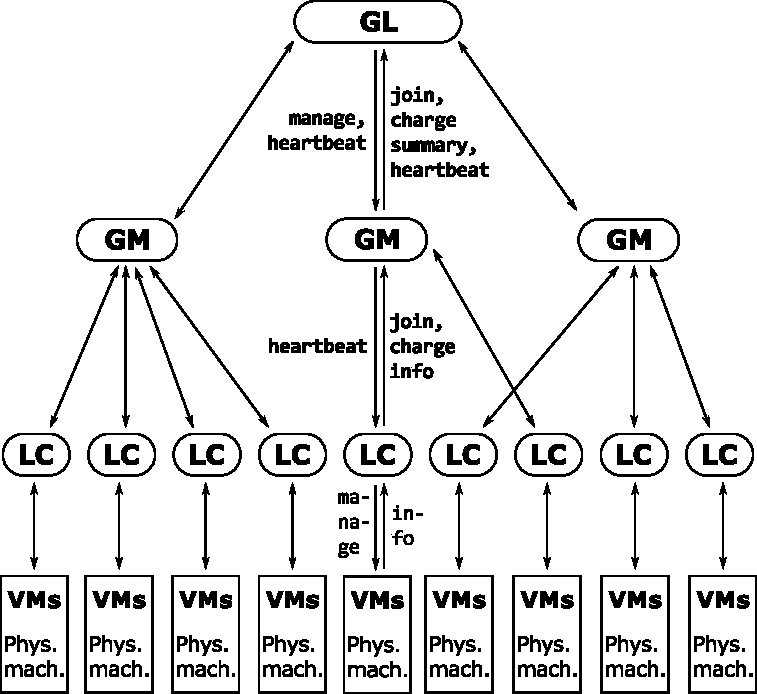
\includegraphics[width=.95\linewidth]{figures/snoozearch.pdf}}
  \caption{Overview of Snooze's architecture}
  \label{fig:snoozearch}
\end{figure}

\paragraph{Architecture}

Snooze harnesses a hierarchical architecture in order to support load
balancing and fault tolerance, see Fig.~\ref{fig:snoozearch}. At the
top of the hierarchy, a \emph{group leader (GL)} (that is installed on
a service node in our simulation) centralizes information about the
whole cluster by keeping summary information about all \emph{group
  managers (GMs)} (also installed on service nodes in our simulation)
that constitute the intermediate layer of the hierarchy. GMs manage a
number of \emph{local controllers (LCs)} (installed on an ordinary
node) and manages the VMs assigned to that node. During execution,
higher-level components periodically send heartbeats to lower-level
components; monitoring information, \eg on the system load, is also
sent periodically in the opposite direction. In order to propagate
information down the hierarchy, Snooze relies on hardware support for
multicast communication. Finally, a number of replicated entry points
allows clients to contact the GL, \eg in order to submit new VMs for
integration into the system.

\paragraph{Algorithms}
\label{sec:snoozeAlgs}

Apart from the handling of faults (described below), two types of
algorithms are of major importance for the administration of the
Snooze architecture: the algorithms that enable components to
dynamically enter the system and the algorithms that propagate info
between the components.

A GL is created, if it does not exist, by promotion of a GM that is
selected according to some leader election algorithm. When a GM joins
a cluster, it starts listening on a predefined channel for the
heartbeat of the GL and registers once it has received the
heartbeat. New LCs first also wait for the GL heartbeat, request a GM
assignment from the GL and register at the GM assigned to them.

Information that is passed within the system consists in periodic
heartbeat message from the GL, GMs and LCs as well as, also periodic,
charge information from LCs sent to their respective GMs and summary
charge info sent by GMs to the GL.


\paragraph{Fault tolerance}

GLs, GMs and LCs may fail during the system execution. System
components identify that a node on the corresponding higher-level node
has failed (the GL in case of a GM, a GM in the case of an LC) in an
asynchronous fashion through the lack of heartbeat messages.

In the case of a GL failure, one of the GMs becomes the new GL, stops
its GM activities and prevents the LCs it manages so that they can
start rejoining the system. If a GM fails, the GL and the LCs it has
managed will become aware of it based on the lack of heartbeats,
update its data structures and, for the LCs, rejoin the system. If an
LC fails, its GM will finally learn of it due to the missing heartbeat
and charge information of the LC. The GM will then remove the LC from
its data structures.

\subsubsection{Simulation using Simgrid}

Snooze can be simulated using our model and tool support in a direct
and natural manner. The extended abstractions \MS[MS]{Refer to
  Sec.~\ref{sec:overview}} for hosts (\texttt{XHOST}) and VMs
(\texttt{XVM}) provide low-level facilities for scheduling algorithms
that facilitate the implementation of the Snooze simulation. We have
harnessed these facilities in order to implement core characteristics
of Snooze: the monitoring of all VMs that are part of an LC and the
migration of all VMs of the set of LCs that are managed by a GM.

The remaining concepts and algorithms of Snooze are implemented using
means of our framework, the facilities provided by Simgrid and
standard Java mechanisms. Communication between Snooze actors is
implemented based on Simgrid's primitives for, mainly asynchronous,
event handling; in particular, hardware-supported multicast
communication that is used, for example, in order to relay heartbeats
is implemented as a dedicated actor that manages a state representing
GL and GM heartbeat groups and relaying heartbeat events.

The Snooze simulation uses, as its original counterpart, a
multi-threaded implementation in order to optimize reactivity even for
large groups of LCs (or GMs) that have to be managed by one GM (or
GL).

\subsubsection{Variants}
\label{sec:snoozeVariants}

Our simulation framework facilitates the simulation of variants of
placement algorithms. In the following, we present three non-trivial
variants that we have implemented and explored: a variant of the
assignment algorithm of LCs to GMs, periodic vs.\ reactive scheduling,
and a variant of the algorithms of how GMs and LCs join the system.


\paragraph{Assignment of LCs to GMs}

LCs are assigned to GMs by the GL as part of the LC join protocol. In
Snooze's native implementation LCs are assigned in a round-robin
fashion to the known GMs. If GMs join (and leave) the system at the
same time as LCs, a round-robin strategy at join time, however, does
not ensure an even distribution. This may happen, for instance at
startup time of the system, when new GMs and LCs enter the system, or
in case of failures, which trigger GM and LC joins. In order to
evaluate the imbalance resulting from a round-robin strategy (as well
as others) we have implemented the LC assignment protocol in a modular
fashion and applied it in diverse highly-dynamic settings in which GMs
and LCs enter the system at the same time. Furthermore, we have
implemented a best-fit strategy that assigns LCs to GMs with minimal
load or to GMs with the smallest number of assigned LCs (if several
GMs with minimal load exist). The best-fit strategy can significantly
improve the scheduling characteristics of hierarchical placement
algorithms as shown by the experimental data presented in
Sec.~\ref{sec:snoozeVariantsEval}. Furthermore, it should always be
at least as good as the round-robin strategy (the corresponding proof
is left to future work).


\paragraph{Periodic vs.\ reactive scheduling}

Snooze~\cite{feller:ccgrid12} schedules VMs in a periodic fashion:
after a fixed time period a GM calls the scheduler in order to resolve
resource conflicts among the LCs it manages. The information whether a
resource conflict has to be handled is taken based on the summary
information that is periodically sent by the LCs to the GM.

We have provided an alternative, reactive, strategy to scheduling: as
soon as they occur, LCs avert their GMs of resource conflicts; the GMs
then initiate scheduling. Implementing this reactive scheme can be
done using our framework in two manners: either by implementing
additional asynchronous transmissions as a real implementation of the
necessary state updates would proceed or, in a much more lightweight
manner, through direct accesses by the GMs to the states of their
respective LCs. While the latter does not mimic a real implementation
closely, it can be harnessed to yield a valid simulation: delays
induced by communication in the ``real'' implementation, for instance,
can be easily added as part of the lightweight simulation. We have
implemented this lightweight variant of reactive scheduling.


\paragraph{Variants of the join algorithms}

The join algorithms, see Sec.~\ref{sec:snoozeAlgs}, are crucial to the
correctness of Snooze for two main reasons: (i) they have to be
efficient because they can easily form a bottleneck if large numbers
of LCs (GMs) have to be registered at a GM (LC); (ii) they are
multi-phase protocols whose correctness especially in the presence of
faults is difficult to ensure.

In order to investigate the corresponding trade-offs, we have used our
framework to implement join algorithms that may be interrupted at any
time, repeat the the on-going phase a number of times before
reinitiating, if necessary, the entire protocol. Furthermore, the join
protocol is parameterized, \eg, in the number of threads used to
handle registration requests.

Finally, our framework has enabled us to test another aspect of
Snooze's join algorithm as presented by
Feller~\etal.~\cite{feller:ccgrid12},
\MS[MS]{If we succeed to perform the experiment comparing both
  approach, this paragraph should be highlighted.}
a strategy we call the GM rejoin
strategy (GRJ): all GMs should rejoin if a new GM enters the
system. While GRJ supports a form of load balancing (because all LCs
are reassigned to the new set of GMs), our simulation has shown that
this strategy significantly increases the time necessary for
registering GMs and LCs compared to a simpler strategy that does not
modify existing GMs in case a new GM enters the system. This handicap
is particularly pronounced if joins of GMs may be interrupted due to
faults. Concretely, experiments involving 20 GMs and 200 LCs have
shown that this strategy often multiplies the time necessary to join
all 220 components by 10 or more compared to the simple join
strategy. While the qualitative result that the more complex strategy
presented in the paper results in a more time-consuming join process
is not very surprising, the extent of the resulting degradation was
surprising.



%%% Local Variables:
%%% mode: latex
%%% TeX-master: "main"
%%% End:


\subsection{DVMS}
\label{subsec:dvms}
\AL[AL]{Check who write that part, If Flavien did it, then add him as
  an author}
% As the third use-case, we have implemented the
DVMS (Distributed Virtual Machine Scheduler)~\cite{quesnel:cpe2012} enables the
cooperative and fully-distributed placement of
VMs. A DVMS agent is deployed on each node in order to manage the VMs on
the node and collaborate with (the agents of) neighboring nodes.
Agents are defined on top of an overlay communication network that
defines the node-neighbor relation.
% and can be structured (using, \eg
% Chord~\cite{stoica:2001:sigcomm01}) or unstructured.  For this
% study,
We have implemented a simple % but effective
unstructured overlay that enables the agents to collaborate
% without side effects: when necessary, \eg in case of node failures,
% the overlay
by providing a link to a neighbor %of a node
on the latter's request.
% \MS[AL, JP]{A bit short. What about an architecture figure (as for
%  Snooze?)}




% \paragraph{Iterative Scheduling Procedure.}
% \label{sec:ISP}
% \AL[MS,JP]{if we succeed to have only one or two subsections in
%   Snooze, we should do the same here.}

Fig. \ref{fig:dvms_pte} depictes the DVMS algorithm.
When a node N\(_{\textit{i}}\) detects that it cannot provide enough
resources for its hosted VMs, %(\ie VMs hosted on the server require more
%resources than available),
an \emph{Iterative Scheduling Procedure
  (ISP}) is started:
%
%When a node N\(_{\textit{i}}\)
%detects that it cannot provide enough resources for its hosted VMs,
it initiates a partition, reserving itself to solve the problem (sse
Fig.~\ref{fig:dvms_pte_1}).
Then, its
closest neighbor % , as defined by the network overlay,
is considered.
%
%
%
If this neighbor, N\(_{\textit{i+1}}\),
is already part of another partition, the next neighbor is considered.
%\AL[MS]{Not clear enough, its next neighbor ?}
Otherwise, N\(_{\textit{i+1}}\)
joins the partition (see Fig.~\ref{fig:dvms_pte_2}) and becomes the
partition leader.
% % If the partition is not valid anymore (\eg because the workload of the
% % partition's VM has decreased), N\(_{\textit{i+1}}\)
% % cancels the reservations, destroys the partition and thus frees its
% % nodes for another problem solving procedure.
% % %
% % On the contrary, if the procedure is still valid, N\(_{\textit{i+1}}\)
% % notifies members of the partition that it has become the new
% % leader.
%
The other nodes involved in the partition then send it information about their
capacities and current load. The leader, in turn, starts a scheduling
computation looking for a reconfiguration within the current
partition. If no solution is found, the same algorithm is applied to
the next node N\(_{\textit{i+2}}\).
%
% % In the extreme case a partition may grow until all resources in a
% % cluster contribute to the resolution of its resource scheduling
% % problem.
This approach constructs small parititions in a highly parallel
manner (Fig.~\ref{fig:dvms_pte_3}), thus significantly accelerating
the scheduling process and thus the reactivity criteria.

Most of the DVMS code has been coded in SCALA leveraging the Java
primitives of \sg for the communications between the different DVMS agents.

\begin{figure}[t]
\vspace*{-.6cm}
\subfigure[]{
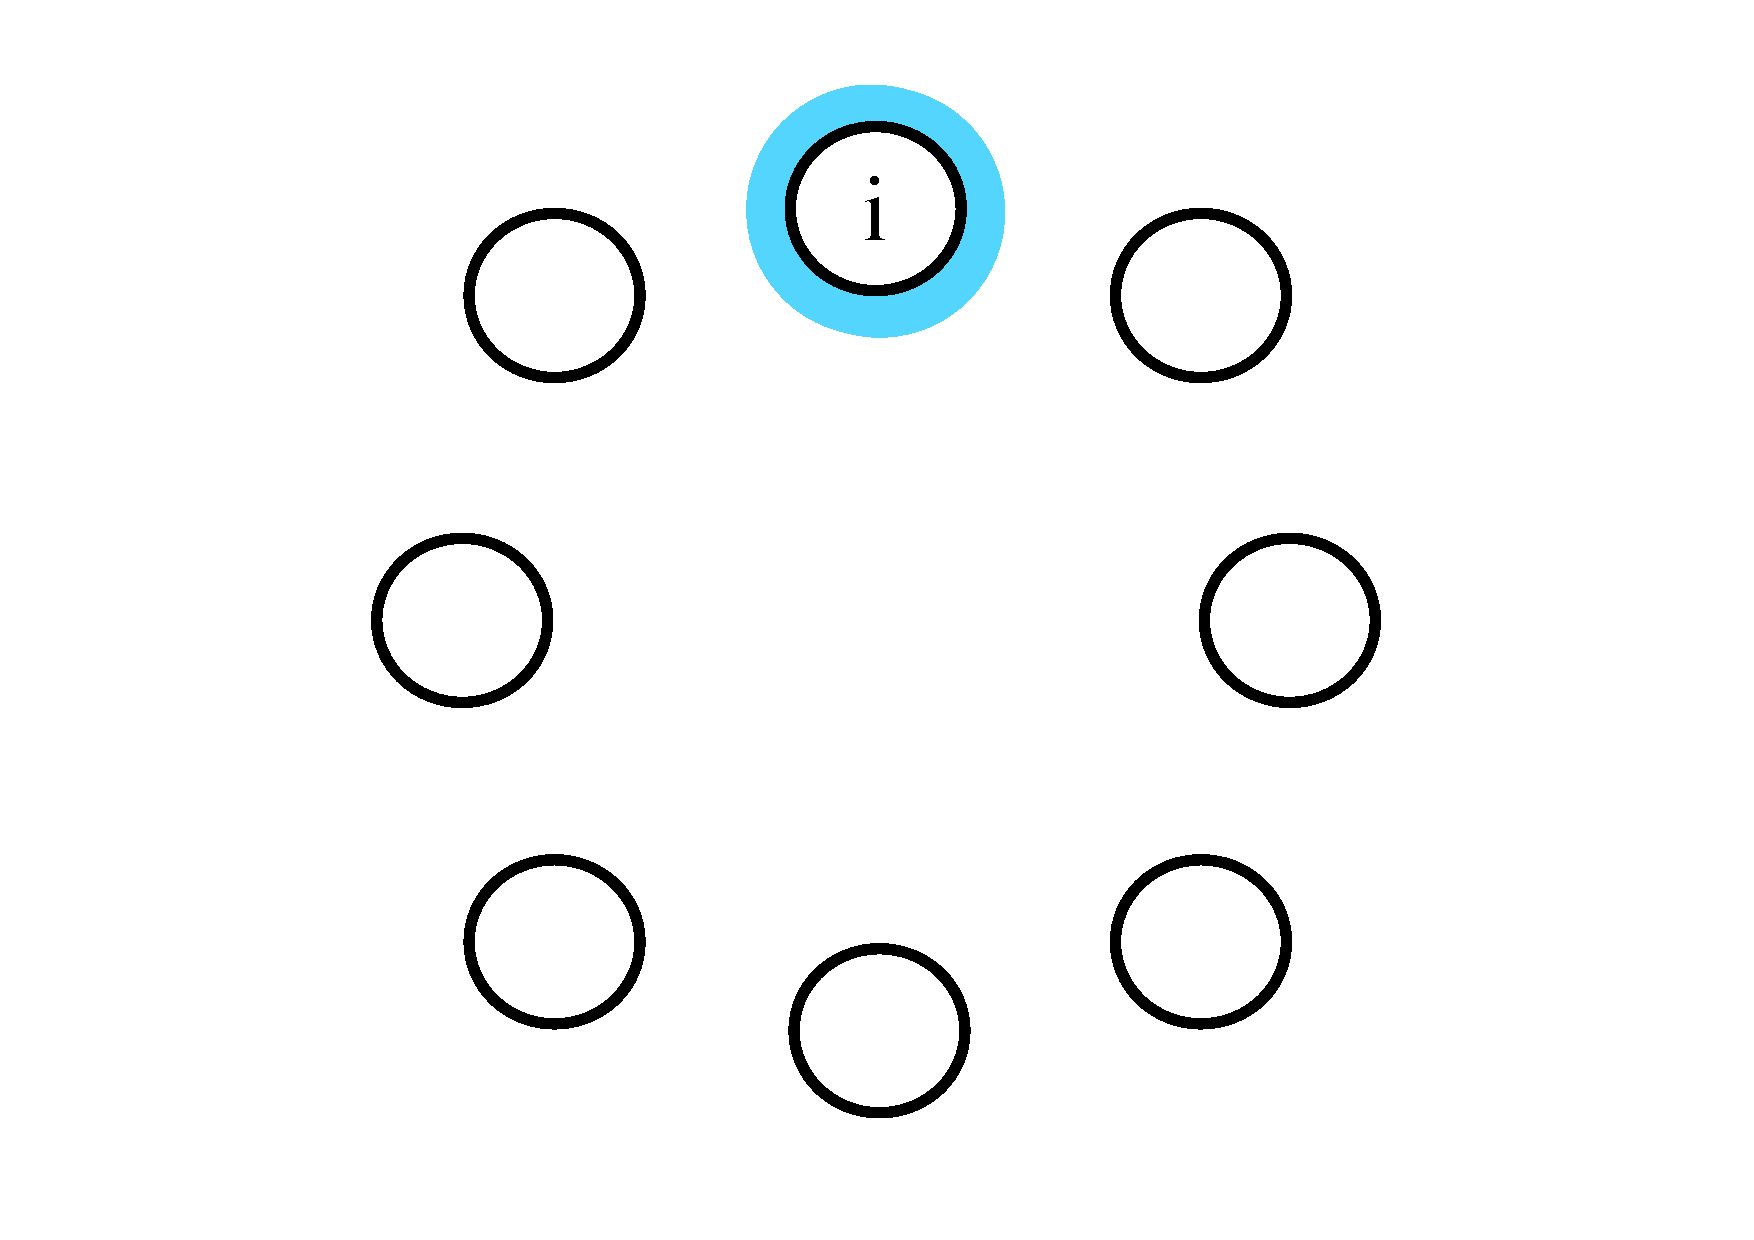
\includegraphics[width=2.7cm]{./figures/fig-24.pdf}
\label{fig:dvms_pte_1}}
%
\subfigure[]{
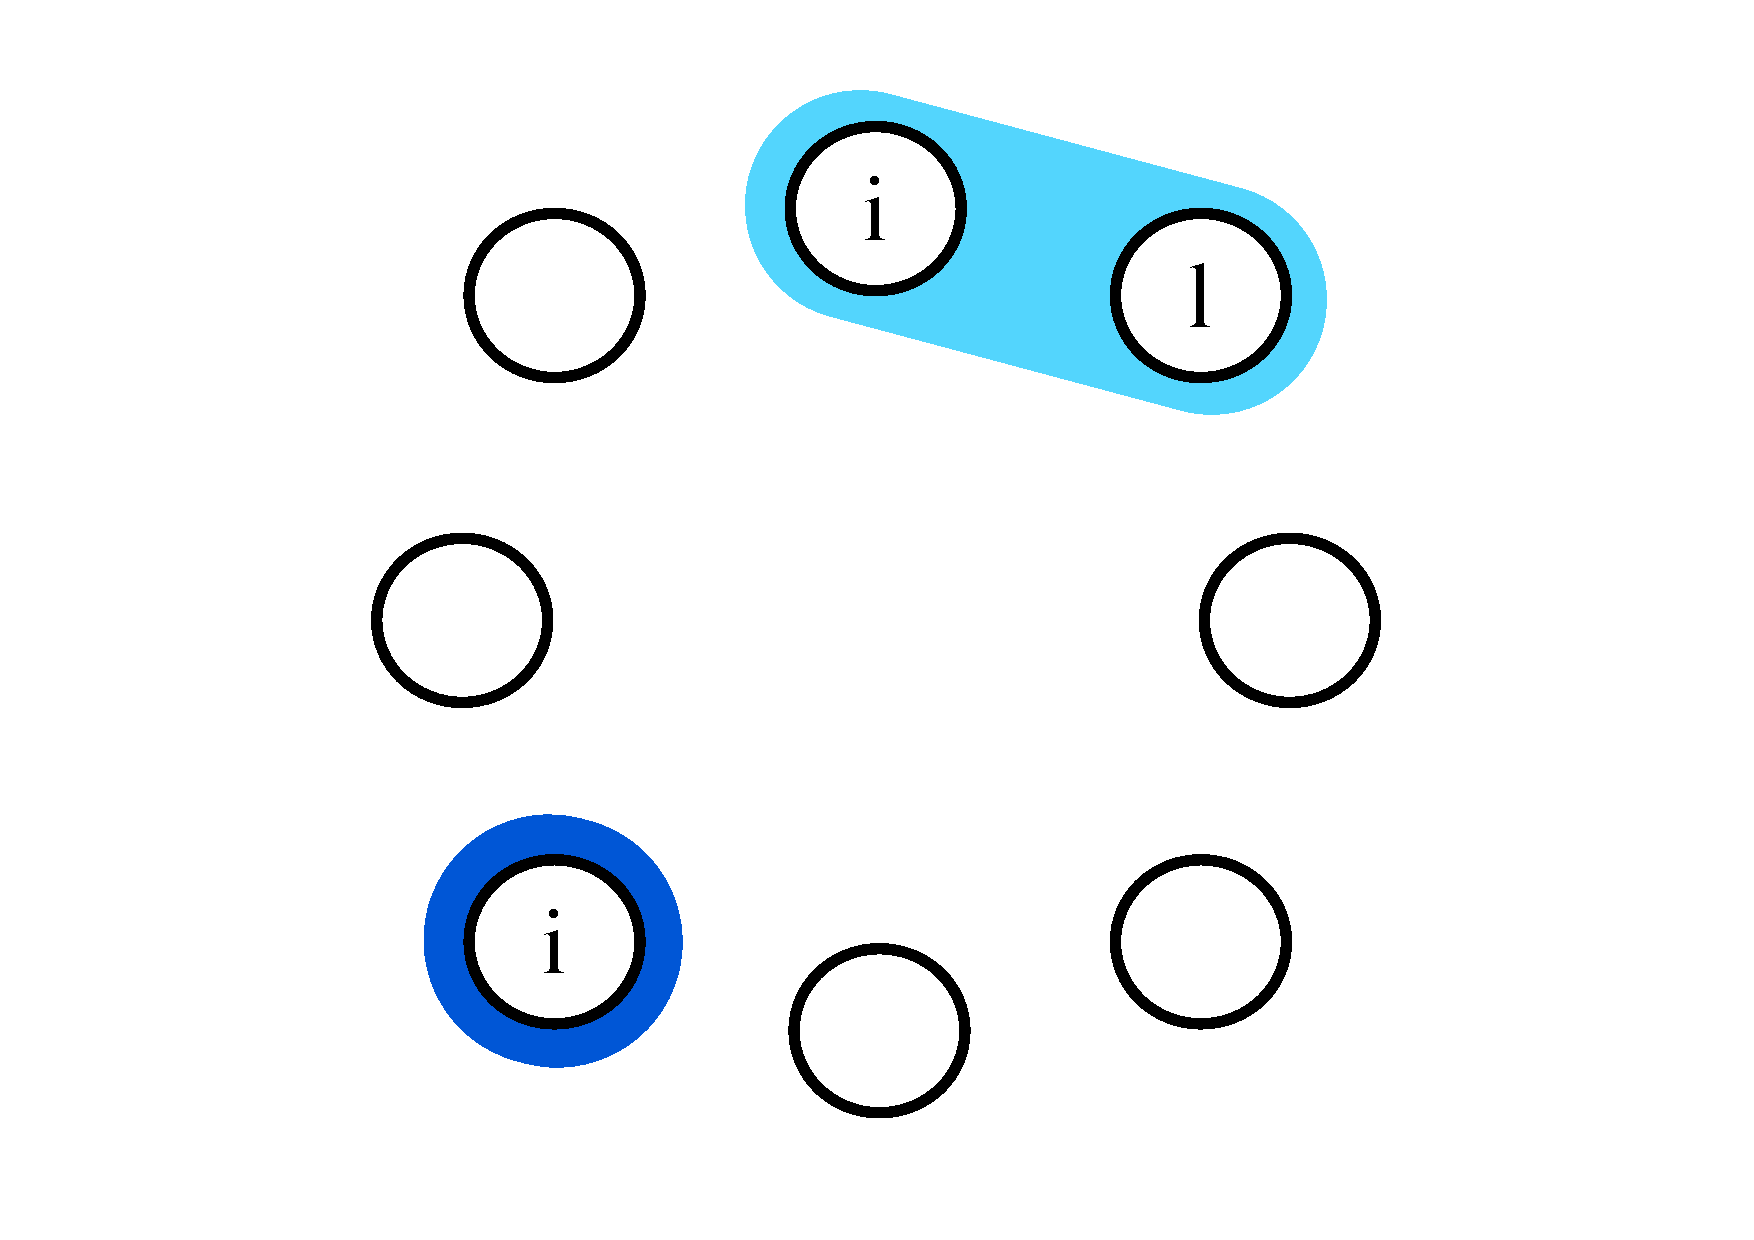
\includegraphics[width=2.7cm]{./figures/fig-25.pdf}
\label{fig:dvms_pte_2}}
%
\subfigure[]{
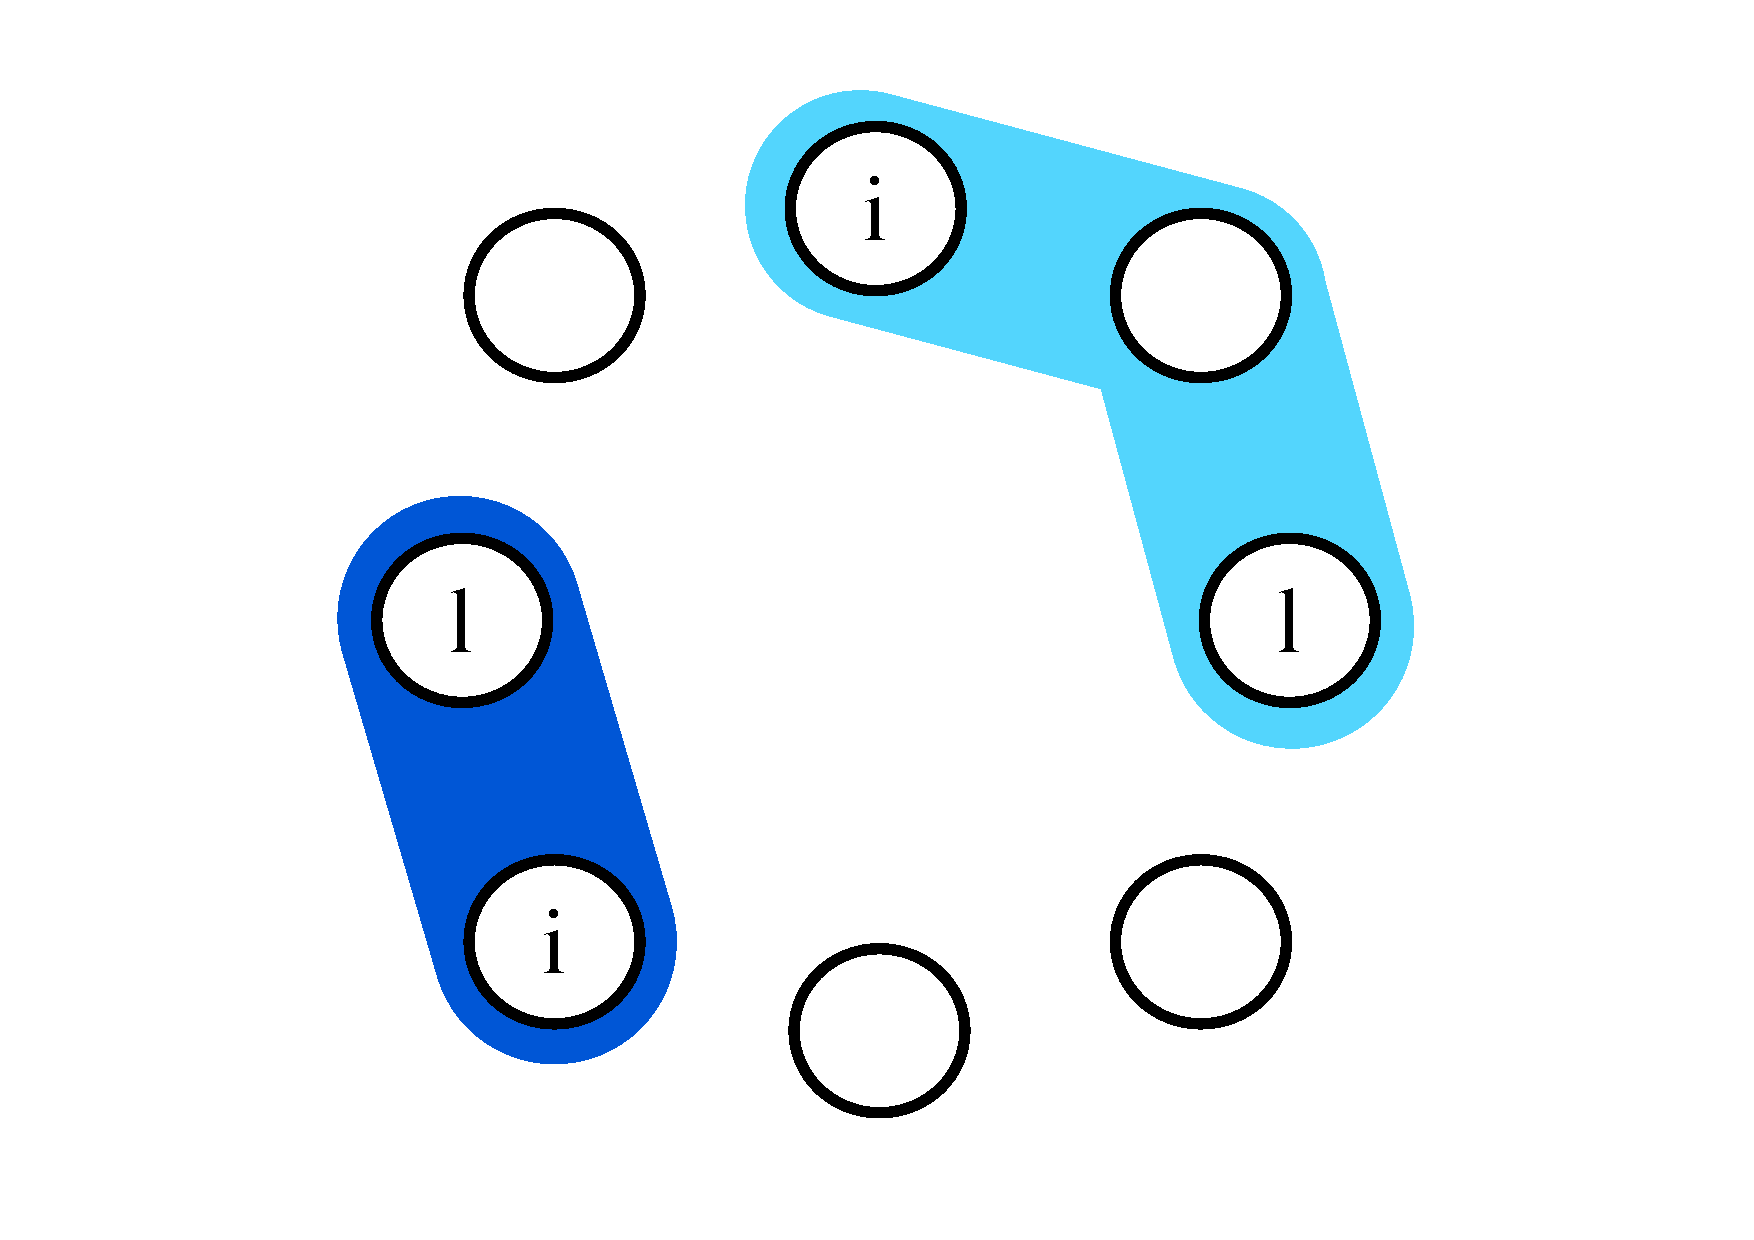
\includegraphics[width=2.7cm]{./figures/fig-26.pdf}
\label{fig:dvms_pte_3}}
%
\subfigure[Legend]{
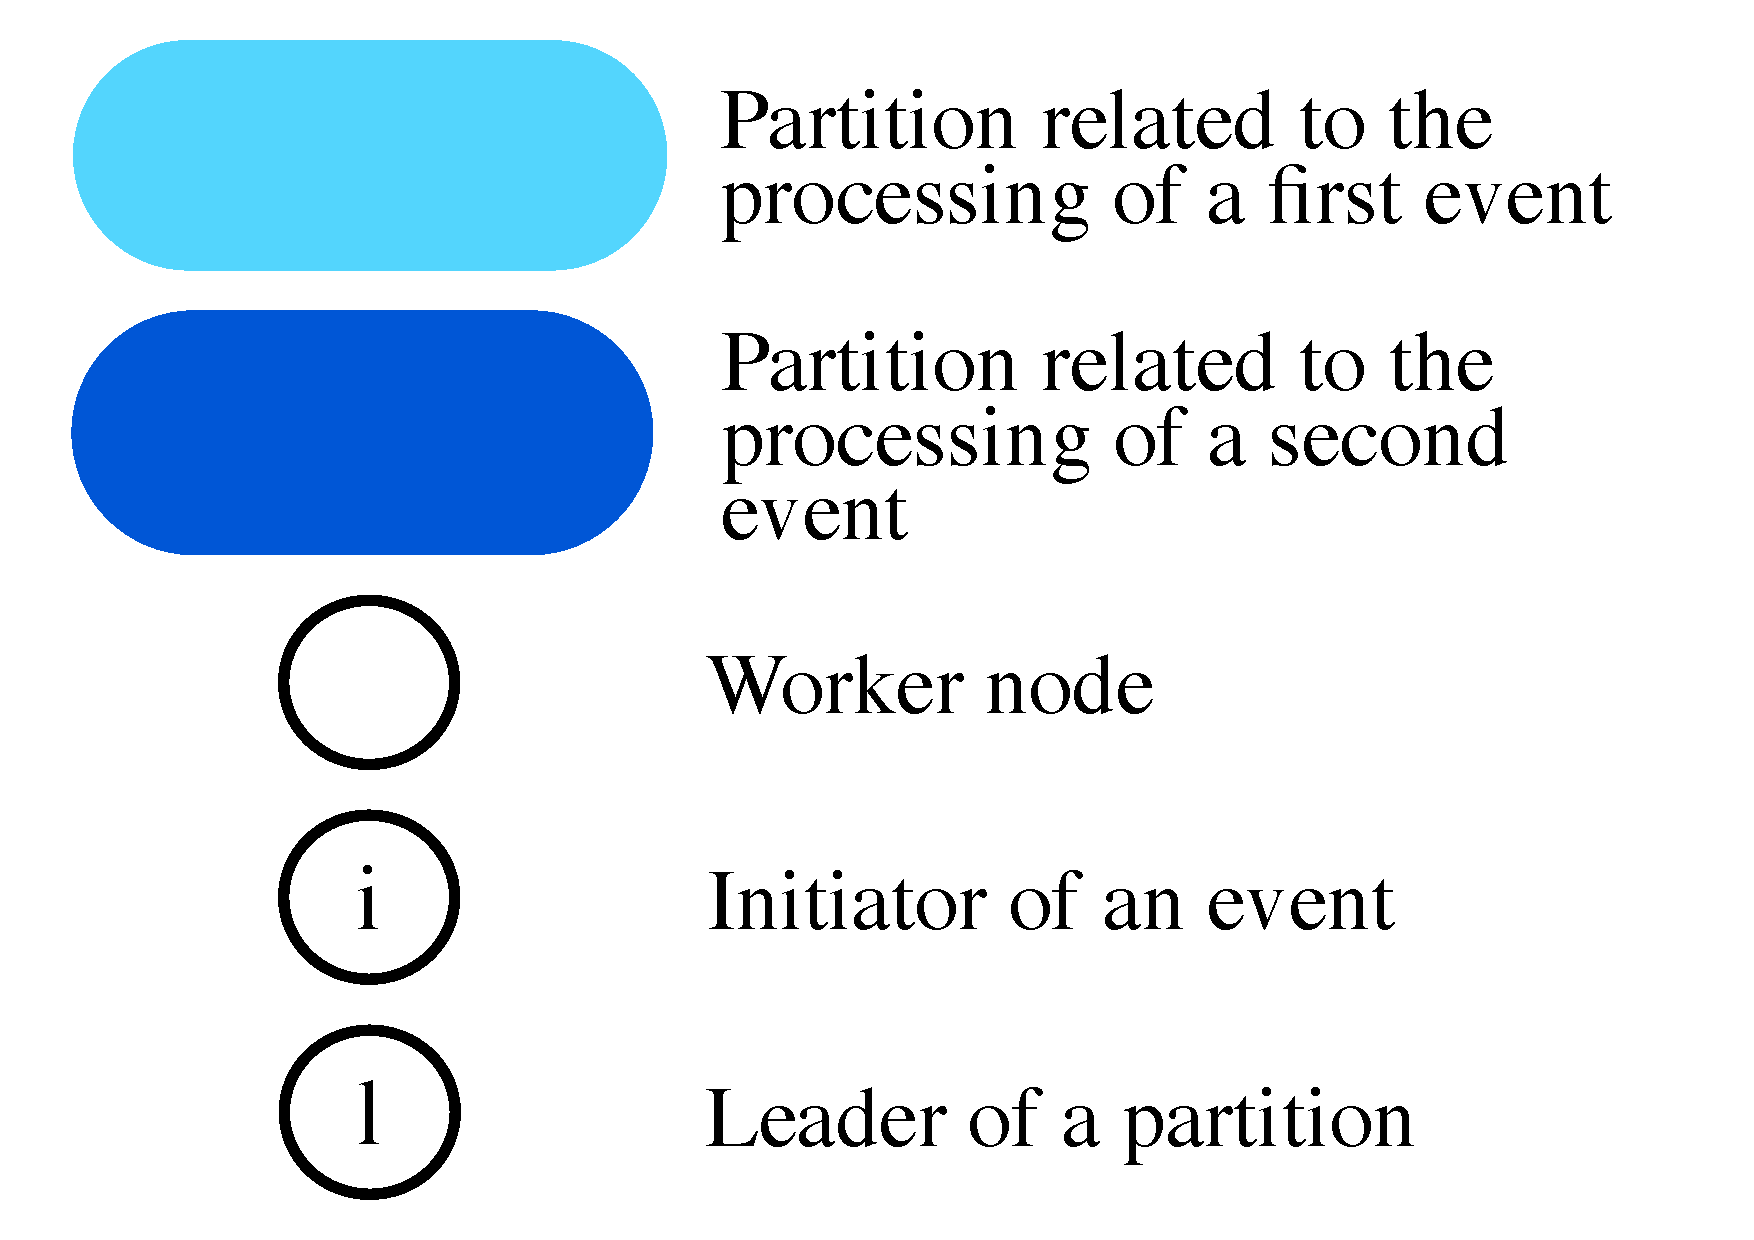
\includegraphics[width=2.7cm]{./figures/fig-27.pdf}
\label{fig:dvms_pte_4}}
%
\vspace*{-.3cm}
\caption{Processing two events simultaneously\label{fig:dvms_pte}}
\vspace*{-.6cm}
\end{figure}


% \subsubsection{Fault-tolerance}

% The main advantage of using overlay networks is that they have
% built-in fault tolerance mechanisms. DVMS therefore works on top of an
% overlay network such as Chord: when a node needs to rebalance its VMs
% workload, it uses the overlay network to find collaborators. For this
% study we implemented a simple overlay network as a flat list of
% agents: a typical request for collaborators includes the list of
% agents that are already collaborating with the requesting agent. A
% link to a new collaborator is then provided to the requesting
% agent. Communication is performed by message exchanges containing
% immutable data: our implementation harnesses the principles of the
% actor model in order to ease the handling of concurrency and
% distributed issues.

% Even if the implementation of the overlay network is simple, it
% fulfills its purpose, and in the case where one would want to use a
% different overlay network such as a ring topology, it only has to
% reuse the API provided by this simple implementation, and adapts its
% functionning to the targeted overlay network.
% \AL[JP]{here we do not describe DVMS in general but we should
% emphasize what has been exactly implemented and how} \JP[AL]{I added
% the preceding paragraph that gives more details about the overlay
% network used.}
%
% This functionning allows firstly a loosely coupling between DVMS and
% the overlay network used, and, secondly, to delegate most of the
% fault tolerance mechanisms to the overlay network. Although
% leveraging an overlay network to address node crashes is helpfull,
% it is not enough to make the problem solving procedure
% fault-tolerant.

% Harnessing the fault tolerance mechanisms of the underlying overlay
% network is, however, not sufficient. If the leader of a partition
% crashes, a new leader must take over in order for the resource problem
% to be solved and the nodes of a partition to be finally freed.  To
% avoid these issues, DVMS now relies on timeout mechanisms.  Each node
% of a partition periodically checks whether the state of its partition
% changed recently (\eg, if a new node joined the partition) and can
% thus identify if the partition's leader is not active anymore.  In
% this case, each node leaves the partition and can be integrated in
% other partitions.

%%% Local Variables:
%%% mode: latex
%%% TeX-master: "main"
%%% End:

\section{Experiments}
\label{sec:experiments}
\AL[JP,AL,MS]{2 pages}
\AL{Il faudra parler du nombre de migrations qui est egalement une
  métrique pertinente. Plusieurs algorithms tentent de reduire cette
  metrique }
\section{Related Work}
\label{sec:related}
\AL[AL]{.25 page}
\section{Conclusion}
\label{sec:conclusion}
\AL[AL]{.25 page}



% conference papers do not normally have an appendix


% use section* for acknowledgement
\section*{Acknowledgment}
This work is supported by the French ANR project SONGS (11-INFRA-13).


\bibliographystyle{wileyj}
\bibliography{main}

\end{document}

%%% Local Variables:
%%% mode: latex
%%% TeX-master: "main"
%%% End:
